%===============================================================================
% MPMD & MPI Runtime Infrastructure in NOAA Global Workflow
% Comprehensive Technical Specification
%===============================================================================
\documentclass[11pt,a4paper,twoside]{article}

%-------------------------------------------------------------------------------
% Package Imports
%-------------------------------------------------------------------------------
\usepackage[utf8]{inputenc}
\usepackage[T1]{fontenc}
\usepackage{lmodern}
\usepackage{amsmath,amssymb,amsfonts}
\usepackage{graphicx}
\usepackage{xcolor}
\usepackage{hyperref}
\usepackage{booktabs}
\usepackage{longtable}
\usepackage{tabularx}
\usepackage{float}
\usepackage{fancyhdr}
\usepackage{listings}
\usepackage{algorithm}
\usepackage{algorithmic}
\usepackage{tikz}
\usepackage{geometry}
\usepackage{parskip}
\usepackage{caption}
\usepackage{subcaption}
\usepackage{enumitem}
\usepackage{fancyvrb}
\usepackage{url}
\usepackage{natbib}

%-------------------------------------------------------------------------------
% TikZ Libraries
%-------------------------------------------------------------------------------
\usetikzlibrary{shapes,arrows,positioning,fit,backgrounds,calc}

%-------------------------------------------------------------------------------
% Page Geometry
%-------------------------------------------------------------------------------
\geometry{
    a4paper,
    left=25mm,
    right=25mm,
    top=30mm,
    bottom=30mm
}

%-------------------------------------------------------------------------------
% Color Definitions
%-------------------------------------------------------------------------------
\definecolor{noaablue}{RGB}{0,51,102}
\definecolor{noaagold}{RGB}{255,195,0}
\definecolor{codebg}{RGB}{248,248,248}
\definecolor{codeframe}{RGB}{200,200,200}
\definecolor{keywordcolor}{RGB}{0,0,180}
\definecolor{stringcolor}{RGB}{0,128,0}
\definecolor{commentcolor}{RGB}{128,128,128}

%-------------------------------------------------------------------------------
% Hyperref Setup
%-------------------------------------------------------------------------------
\hypersetup{
    colorlinks=true,
    linkcolor=noaablue,
    filecolor=magenta,
    urlcolor=noaablue,
    citecolor=noaablue,
    pdftitle={MPMD \& MPI Runtime Infrastructure in NOAA Global Workflow},
    pdfauthor={MCP/RAG Analysis System},
    pdfsubject={HPC Infrastructure Technical Specification},
    pdfkeywords={MPI, MPMD, HPC, Global Workflow, NOAA, GFS, Weather Forecasting}
}

%-------------------------------------------------------------------------------
% Code Listing Style
%-------------------------------------------------------------------------------
\lstdefinestyle{bashstyle}{
    language=bash,
    basicstyle=\ttfamily\small,
    backgroundcolor=\color{codebg},
    frame=single,
    rulecolor=\color{codeframe},
    keywordstyle=\color{keywordcolor}\bfseries,
    stringstyle=\color{stringcolor},
    commentstyle=\color{commentcolor}\itshape,
    breaklines=true,
    breakatwhitespace=true,
    numbers=left,
    numberstyle=\tiny\color{gray},
    numbersep=5pt,
    showstringspaces=false,
    tabsize=2,
    captionpos=b,
    morekeywords={export,source,module,load,srun,mpiexec,cfp}
}

\lstdefinestyle{luastyle}{
    language=[5.2]Lua,
    basicstyle=\ttfamily\small,
    backgroundcolor=\color{codebg},
    frame=single,
    rulecolor=\color{codeframe},
    keywordstyle=\color{keywordcolor}\bfseries,
    stringstyle=\color{stringcolor},
    commentstyle=\color{commentcolor}\itshape,
    breaklines=true,
    numbers=left,
    numberstyle=\tiny\color{gray},
    numbersep=5pt,
    showstringspaces=false,
    tabsize=2,
    morekeywords={load,setenv,prepend_path,depends_on}
}

%-------------------------------------------------------------------------------
% Header and Footer
%-------------------------------------------------------------------------------
\pagestyle{fancy}
\fancyhf{}
\fancyhead[LE,RO]{\thepage}
\fancyhead[LO]{\nouppercase{\rightmark}}
\fancyhead[RE]{\nouppercase{\leftmark}}
\fancyfoot[C]{\small NOAA Global Workflow Technical Specification}
\renewcommand{\headrulewidth}{0.4pt}
\renewcommand{\footrulewidth}{0.4pt}

%-------------------------------------------------------------------------------
% Title Page Information
%-------------------------------------------------------------------------------
\title{%
    \vspace{1cm}
    {\Huge\bfseries\color{noaablue} MPMD \& MPI Runtime Infrastructure\\[0.3cm]
    in NOAA Global Workflow}\\[0.5cm]
    {\Large\itshape Comprehensive Technical Specification}\\[0.5cm]
    {\large Version 1.0}
}

\author{%
    \textbf{MCP/RAG Analysis System}\\
    NOAA Environmental Modeling Center\\
    National Centers for Environmental Prediction\\[0.5cm]
    \texttt{global-workflow@noaa.gov}
}

\date{January 30, 2026}

%===============================================================================
\begin{document}
%===============================================================================

\maketitle
\thispagestyle{empty}

%-------------------------------------------------------------------------------
% Abstract
%-------------------------------------------------------------------------------
\begin{abstract}
\noindent
The Global Workflow, maintained by NOAA's Environmental Modeling Center (EMC), implements production weather forecasting systems including the Global Forecast System (GFS), Global Ensemble Forecast System (GEFS), Seasonal Forecast System (SFS), and Global Composition/Chemistry Aerosol Forecast System (GCAFS). Central to this infrastructure is a sophisticated \textbf{Multi-Program Multiple-Data (MPMD)} execution framework that enables heterogeneous parallel task execution across diverse high-performance computing (HPC) platforms.

This technical specification provides a comprehensive analysis of the MPMD architecture, MPI runtime configurations, and platform-specific optimizations that enable the Global Workflow to execute efficiently on eleven distinct HPC systems---from NOAA's operational WCOSS2 production environment to research platforms including Hera, Hercules, Orion, and Gaea, as well as cloud-based ParallelWorks deployments on AWS, Azure, and Google Cloud.

The document covers the core \texttt{run\_mpmd.sh} orchestration script, the three-level job resource configuration chain, platform-specific MPI tuning parameters, network fabric optimizations, and the critical \textbf{Coupled Framework Parallelism (CFP)} module used exclusively on WCOSS2. We present the complete environment variable taxonomy, command file format transformations, and troubleshooting procedures essential for operational reliability.
\end{abstract}

\vspace{1cm}

%-------------------------------------------------------------------------------
% Keywords
%-------------------------------------------------------------------------------
\noindent\textbf{Keywords:} MPI, MPMD, HPC, Global Workflow, NOAA, GFS, GEFS, WCOSS2, Slurm, PBS, Intel MPI, Cray MPICH, CFP, Slingshot, InfiniBand

\newpage
\tableofcontents
\newpage
\listoffigures
\listoftables
\newpage

%===============================================================================
\section{Introduction}
\label{sec:introduction}
%===============================================================================

The National Oceanic and Atmospheric Administration (NOAA) operates some of the world's most sophisticated numerical weather prediction systems. At the core of these systems lies the \textbf{Global Workflow}---an integrated software framework that orchestrates the execution of complex forecast cycles across multiple high-performance computing (HPC) platforms.

\subsection{Problem Statement}

Modern weather forecasting requires executing thousands of heterogeneous tasks with varying computational characteristics:

\begin{itemize}[noitemsep]
    \item \textbf{Embarrassingly parallel tasks}: Observation processing, post-processing, product generation
    \item \textbf{Tightly coupled tasks}: Model forecast integration requiring MPI collective operations
    \item \textbf{I/O intensive tasks}: Data staging, archive operations, file transformations
\end{itemize}

The challenge is executing these diverse workloads efficiently across platforms with fundamentally different:
\begin{itemize}[noitemsep]
    \item Job schedulers (Slurm vs. PBS Pro)
    \item MPI implementations (Intel MPI, Cray MPICH, PMI2)
    \item Network fabrics (InfiniBand, Slingshot, EFA)
    \item File systems (Lustre, GPFS)
\end{itemize}

\subsection{Solution Architecture}

The Global Workflow implements a \textbf{platform abstraction layer} that provides:

\begin{enumerate}
    \item \textbf{Unified MPMD Interface}: The \texttt{run\_mpmd.sh} script accepts a generic command file and transforms it to platform-specific format
    \item \textbf{Three-Level Configuration}: Base resources, platform overrides, and environment binding
    \item \textbf{Launcher Abstraction}: Platform-specific \texttt{\$launcher} and \texttt{\$mpmd\_opt} variables
    \item \textbf{Module Environment}: Lua modulefiles for runtime library loading
\end{enumerate}

\subsection{Document Scope}

This specification covers:
\begin{itemize}[noitemsep]
    \item Complete MPMD execution flow from job script to MPI ranks
    \item All eleven supported HPC platforms and their configurations
    \item MPI tuning parameters for Intel MPI and Cray MPICH
    \item Network fabric optimizations (InfiniBand, Slingshot, EFA)
    \item CFP (Coupled Framework Parallelism) on WCOSS2
    \item Troubleshooting procedures and diagnostic techniques
\end{itemize}

%===============================================================================
\section{Architecture Overview}
\label{sec:architecture}
%===============================================================================

\subsection{System Component Hierarchy}

Figure~\ref{fig:architecture} illustrates the complete MPMD execution architecture.

\begin{figure}[H]
\centering
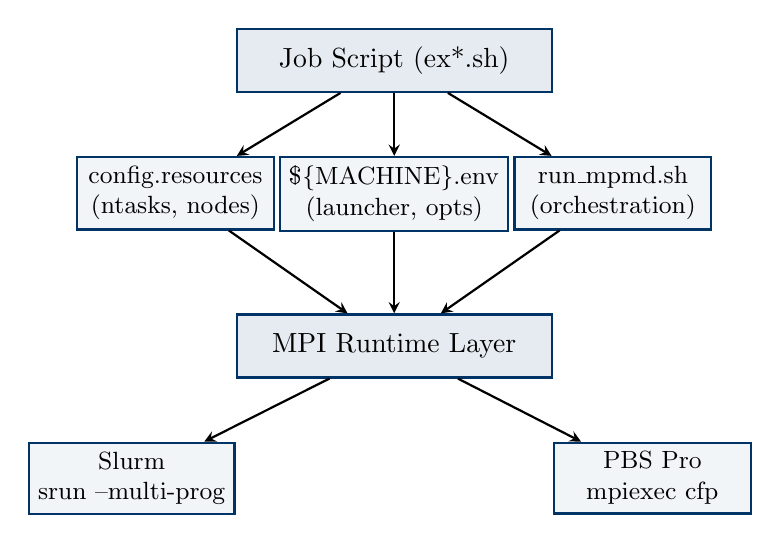
\begin{tikzpicture}[
    node distance=0.8cm,
    box/.style={rectangle, draw=noaablue, fill=noaablue!10, thick, minimum width=4cm, minimum height=0.8cm, align=center},
    smallbox/.style={rectangle, draw=noaablue, fill=noaablue!5, thick, minimum width=2.5cm, minimum height=0.6cm, align=center, font=\small},
    arrow/.style={->, thick, >=stealth}
]

% Top layer
\node[box] (job) {Job Script (ex*.sh)};

% Configuration layer
\node[smallbox, below left=0.8cm and -0.5cm of job] (config) {config.resources\\(ntasks, nodes)};
\node[smallbox, below=0.8cm of job] (env) {\$\{MACHINE\}.env\\(launcher, opts)};
\node[smallbox, below right=0.8cm and -0.5cm of job] (mpmd) {run\_mpmd.sh\\(orchestration)};

% MPI layer
\node[box, below=2.8cm of job] (mpi) {MPI Runtime Layer};

% Platform split
\node[smallbox, below left=0.8cm and 0cm of mpi] (slurm) {Slurm\\srun --multi-prog};
\node[smallbox, below right=0.8cm and 0cm of mpi] (pbs) {PBS Pro\\mpiexec cfp};

% Arrows
\draw[arrow] (job) -- (config);
\draw[arrow] (job) -- (env);
\draw[arrow] (job) -- (mpmd);
\draw[arrow] (config) -- (mpi);
\draw[arrow] (env) -- (mpi);
\draw[arrow] (mpmd) -- (mpi);
\draw[arrow] (mpi) -- (slurm);
\draw[arrow] (mpi) -- (pbs);

\end{tikzpicture}
\caption{Global Workflow MPMD Execution Architecture}
\label{fig:architecture}
\end{figure}

\subsection{Directory Structure}

The MPMD infrastructure is distributed across several key directories:

\begin{lstlisting}[style=bashstyle,caption={MPMD Infrastructure Directory Layout},label={lst:dirs}]
global-workflow/
|-- ush/
|   `-- run_mpmd.sh              # Core MPMD orchestration
|-- env/
|   |-- HERA.env                 # Hera configuration
|   |-- WCOSS2.env               # WCOSS2 configuration
|   |-- GAEAC6.env               # Gaea C6 configuration
|   `-- ...                      # 11 total platforms
|-- dev/
|   |-- parm/config/gfs/
|   |   |-- config.resources     # Base definitions
|   |   `-- config.resources.*   # Platform overrides
|   `-- workflow/hosts/
|       |-- hera.yaml            # Host configuration
|       `-- wcoss2.yaml
`-- modulefiles/
    |-- gw_run.hera.lua          # Hera modules
    `-- gw_run.wcoss2.lua        # WCOSS2 modules
\end{lstlisting}

%===============================================================================
\section{Core MPMD Script Analysis}
\label{sec:run_mpmd}
%===============================================================================

\subsection{Script Overview}

The \texttt{ush/run\_mpmd.sh} script, authored by Rahul Mahajan (NCEP/EMC), serves as the central orchestrator for MPMD execution. It provides a unified interface that adapts to the underlying MPI implementation.

\subsection{Algorithm Description}

Algorithm~\ref{alg:mpmd} presents the complete MPMD execution logic.

\begin{algorithm}[H]
\caption{MPMD Execution Flow}
\label{alg:mpmd}
\begin{algorithmic}[1]
\REQUIRE Command file path \texttt{cmdfile}
\REQUIRE Environment variables: \texttt{USE\_CFP}, \texttt{launcher}, \texttt{mpmd\_opt}, \texttt{DATA}

\STATE \texttt{cmdfile} $\leftarrow$ argument 1

\IF{\texttt{USE\_CFP} $\neq$ ``YES''}
    \STATE Execute \texttt{cmdfile} serially via \texttt{bash}
    \RETURN exit status
\ENDIF

\STATE \texttt{OMP\_NUM\_THREADS} $\leftarrow$ 1 \COMMENT{Force single-threaded for MPMD}
\STATE \texttt{nprocs} $\leftarrow$ line count of \texttt{cmdfile}
\STATE \texttt{mpmd\_cmdfile} $\leftarrow$ \texttt{DATA}/cmdfile.\texttt{RANDOM}

\IF{\texttt{launcher} matches \texttt{``srun.*''}}
    \STATE \COMMENT{Slurm multi-prog format}
    \FOR{each line in \texttt{cmdfile}}
        \STATE Write ``\texttt{rank} \texttt{command}'' to \texttt{mpmd\_cmdfile}
    \ENDFOR
    \STATE Execute: \texttt{launcher} \texttt{mpmd\_opt} -n \texttt{nprocs} \texttt{mpmd\_cmdfile}
    
\ELSIF{\texttt{launcher} matches \texttt{``mpiexec.*''}}
    \STATE \COMMENT{PBS cfp format}
    \STATE Write shebang to \texttt{mpmd\_cmdfile}
    \FOR{each line in \texttt{cmdfile}}
        \STATE Write ``\texttt{command} $>$ mpmd.\texttt{rank}.out 2$>\&$1'' to \texttt{mpmd\_cmdfile}
    \ENDFOR
    \STATE \texttt{chmod 755} \texttt{mpmd\_cmdfile}
    \STATE Execute: \texttt{launcher} -np \texttt{nprocs} \texttt{mpmd\_opt} \texttt{mpmd\_cmdfile}
    
\ELSE
    \STATE Execute \texttt{cmdfile} serially via \texttt{bash}
\ENDIF

\RETURN exit status
\end{algorithmic}
\end{algorithm}

\subsection{Key Implementation Details}

\subsubsection{Thread Control}

MPMD execution forces single-threaded mode:

\begin{lstlisting}[style=bashstyle,caption={Thread Control in MPMD},label={lst:thread}]
export OMP_NUM_THREADS=1
\end{lstlisting}

This ensures each MPI rank executes its assigned serial command without OpenMP parallelism, which would oversubscribe compute resources.

\subsubsection{Launcher Detection}

Pattern matching determines the execution strategy:

\begin{lstlisting}[style=bashstyle,caption={Launcher Pattern Detection},label={lst:launcher}]
if [[ "${launcher:-}" =~ ^srun.* ]]; then
    # Slurm multi-prog execution path
elif [[ "${launcher:-}" =~ ^mpiexec.* ]]; then
    # PBS/CFP execution path
else
    # Serial fallback
fi
\end{lstlisting}

%===============================================================================
\section{HPC Platform Configurations}
\label{sec:platforms}
%===============================================================================

\subsection{Platform Classification}

Table~\ref{tab:platforms} presents the complete platform matrix with scheduler, MPI implementation, and network fabric details.

\begin{table}[H]
\centering
\caption{Global Workflow Supported HPC Platforms}
\label{tab:platforms}
\begin{tabular}{@{}lllll@{}}
\toprule
\textbf{Platform} & \textbf{Scheduler} & \textbf{MPI Library} & \textbf{Network} & \textbf{CFP} \\
\midrule
WCOSS2 & PBS Pro & Cray MPICH & Slingshot & \checkmark \\
Hera & Slurm & Intel MPI & InfiniBand HDR & -- \\
Hercules & Slurm & Intel MPI & InfiniBand & -- \\
Orion & Slurm & Intel MPI & InfiniBand & -- \\
Ursa & Slurm & Intel MPI & InfiniBand & -- \\
Gaea C5 & Slurm & Cray MPICH & Slingshot & -- \\
Gaea C6 & Slurm & Cray MPICH & Slingshot 11 & -- \\
AWS PW & Slurm & PMI2 & EFA & -- \\
Azure PW & Slurm & PMI2 & InfiniBand & -- \\
Google PW & Slurm & PMI2 & VPC Fabric & -- \\
Container & -- & -- & -- & -- \\
\bottomrule
\end{tabular}
\end{table}

\subsection{Tier 1: Production Systems}

\subsubsection{WCOSS2 Configuration}

WCOSS2 (Weather and Climate Operational Supercomputer System, Phase 2) represents NOAA's operational production environment.

\begin{lstlisting}[style=bashstyle,caption={WCOSS2 Launcher Configuration (env/WCOSS2.env)},label={lst:wcoss2}]
# MPI Launcher
export launcher="mpiexec -l"
export mpmd_opt="--cpu-bind verbose,core cfp"

# Thread Configuration
export OMP_PLACES=cores
export OMP_STACKSIZE=1G

# libfabric Tuning
export FI_OFI_RXM_SAR_LIMIT=3145728
export FI_OFI_RXM_RX_SIZE=40000
export FI_OFI_RXM_TX_SIZE=40000

# Collective I/O
export MPICH_MPIIO_HINTS="*:romio_cb_write=enable"
\end{lstlisting}

The WCOSS2 environment uniquely requires the \textbf{CFP module}:

\begin{lstlisting}[style=luastyle,caption={WCOSS2 Runtime Modules (modulefiles/gw\_run.wcoss2.lua)},label={lst:wcoss2mod}]
load("PrgEnv-intel")
load("craype")
load("intel")
load("cray-mpich")
load("cray-pals")
load("cfp")               -- Coupled Framework Parallelism
setenv("USE_CFP", "YES")  -- Enable CFP by default
\end{lstlisting}

\subsection{Tier 2: Research \& Development Systems}

\subsubsection{Hera Configuration}

Hera serves as NOAA's primary R\&D platform.

\begin{lstlisting}[style=bashstyle,caption={Hera Launcher Configuration (env/HERA.env)},label={lst:hera}]
# MPI Launcher
export launcher="srun -l --export=ALL --hint=nomultithread"
export mpmd_opt="--multi-prog --output=mpmd.%j.%t.out"

# Intel MPI Tuning
export MPI_BUFS_PER_PROC=2048
export MPI_BUFS_PER_HOST=2048
export MPI_GROUP_MAX=256
export MPI_MEMMAP_OFF=1
export MP_STDOUTMODE="ORDERED"

# OpenMP Configuration
export KMP_AFFINITY=scatter
export OMP_STACKSIZE=2048000

# Lustre Optimization
export I_MPI_EXTRA_FILESYSTEM=1
export I_MPI_EXTRA_FILESYSTEM_LIST=lustre
\end{lstlisting}

\subsubsection{Gaea C6 Configuration}

Gaea C6 represents the newest NOAA R\&D platform with Slingshot 11 interconnect.

\begin{lstlisting}[style=bashstyle,caption={Gaea C6 Launcher Configuration (env/GAEAC6.env)},label={lst:gaeac6}]
# MPI Launcher with Slingshot optimizations
export launcher="srun -l --export=ALL --distribution=block:block"
export mpmd_opt="--multi-prog --output=mpmd.%j.%t.out"

# Cray Slingshot CXI tuning
export FI_CXI_RX_MATCH_MODE=hybrid
# For large collective-heavy jobs:
# export FI_CXI_RX_MATCH_MODE=software
\end{lstlisting}

\subsection{Tier 3: Cloud Platforms}

\subsubsection{AWS ParallelWorks Configuration}

\begin{lstlisting}[style=bashstyle,caption={AWS ParallelWorks Configuration (env/AWSPW.env)},label={lst:aws}]
# MPI Launcher with PMI2
export launcher="srun -l --export=ALL --hint=nomultithread --mpi=pmi2"
export mpmd_opt="--multi-prog --output=mpmd.%j.%t.out"
\end{lstlisting}

The \texttt{--mpi=pmi2} flag enables PMI2 process management interface, required for MPI on cloud Slurm clusters.

%===============================================================================
\section{MPI Tuning Parameters}
\label{sec:tuning}
%===============================================================================

\subsection{Intel MPI Parameters}

Table~\ref{tab:intelmpi} documents tuning parameters used on Intel MPI platforms.

\begin{table}[H]
\centering
\caption{Intel MPI Tuning Parameters}
\label{tab:intelmpi}
\begin{tabular}{@{}llp{6cm}@{}}
\toprule
\textbf{Variable} & \textbf{Value} & \textbf{Purpose} \\
\midrule
\texttt{MPI\_BUFS\_PER\_PROC} & 2048 & Per-process eager message buffers \\
\texttt{MPI\_BUFS\_PER\_HOST} & 2048 & Per-host shared buffers \\
\texttt{MPI\_GROUP\_MAX} & 256 & Maximum MPI groups \\
\texttt{MPI\_MEMMAP\_OFF} & 1 & Disable memory mapping for IB \\
\texttt{I\_MPI\_ADJUST\_ALLREDUCE} & 5 & GSI-specific allreduce algorithm \\
\texttt{I\_MPI\_EXTRA\_FILESYSTEM} & 1 & Enable parallel filesystem support \\
\texttt{I\_MPI\_EXTRA\_FILESYSTEM\_LIST} & lustre & Optimize for Lustre \\
\bottomrule
\end{tabular}
\end{table}

\subsection{Cray MPICH Parameters}

Table~\ref{tab:craympich} documents parameters for Cray MPICH systems.

\begin{table}[H]
\centering
\caption{Cray MPICH Tuning Parameters}
\label{tab:craympich}
\begin{tabular}{@{}llp{6cm}@{}}
\toprule
\textbf{Variable} & \textbf{Value} & \textbf{Purpose} \\
\midrule
\texttt{FI\_OFI\_RXM\_SAR\_LIMIT} & 3145728 & Segment-and-reassemble limit (3MB) \\
\texttt{FI\_OFI\_RXM\_RX\_SIZE} & 40000 & Receive queue size \\
\texttt{FI\_OFI\_RXM\_TX\_SIZE} & 40000 & Transmit queue size \\
\texttt{FI\_CXI\_RX\_MATCH\_MODE} & hybrid & Slingshot CXI matching mode \\
\texttt{MPICH\_MPIIO\_HINTS} & romio\_cb\_write & Collective buffering for writes \\
\bottomrule
\end{tabular}
\end{table}

\subsection{OpenMP Stack Configuration}

Stack size configuration varies by platform:

\begin{table}[H]
\centering
\caption{OpenMP Stack Configuration by Platform}
\label{tab:stack}
\begin{tabular}{@{}lll@{}}
\toprule
\textbf{Platform} & \textbf{OMP\_STACKSIZE} & \textbf{NTHSTACK} \\
\midrule
WCOSS2 & 1G & -- \\
Hera/Hercules & 2048000 & 1024000000 \\
Gaea C5/C6 & 2048M & -- \\
Forecast jobs & 2048M & -- \\
\bottomrule
\end{tabular}
\end{table}

%===============================================================================
\section{Job Resource Configuration}
\label{sec:resources}
%===============================================================================

\subsection{Three-Level Configuration Chain}

The Global Workflow employs a three-level configuration hierarchy:

\begin{enumerate}
    \item \textbf{Base Resources} (\texttt{config.resources}): Step-agnostic defaults
    \item \textbf{Platform Overrides} (\texttt{config.resources.\$MACHINE}): Machine-specific adjustments
    \item \textbf{Environment Binding} (\texttt{\$MACHINE.env}): Runtime MPI/thread settings
\end{enumerate}

\subsection{Resource Variables}

Table~\ref{tab:resources} defines the standard resource variables.

\begin{table}[H]
\centering
\caption{Job Resource Variables}
\label{tab:resources}
\begin{tabular}{@{}lp{8cm}@{}}
\toprule
\textbf{Variable} & \textbf{Description} \\
\midrule
\texttt{ntasks} & Total MPI tasks requested \\
\texttt{tasks\_per\_node} & MPI tasks per compute node \\
\texttt{max\_tasks\_per\_node} & Hardware maximum (platform-specific) \\
\texttt{threads\_per\_task} & OpenMP threads per MPI task \\
\texttt{memory} & Memory requirement (e.g., ``96GB'') \\
\bottomrule
\end{tabular}
\end{table}

\subsection{APRUN Variable Mapping}

Each job step has a dedicated APRUN variable:

\begin{table}[H]
\centering
\caption{APRUN Variables by Job Step}
\label{tab:aprun}
\begin{tabular}{@{}lll@{}}
\toprule
\textbf{Step} & \textbf{Variable} & \textbf{Configuration} \\
\midrule
fcst & APRUN\_UFS & \texttt{\$launcher -n \$ufs\_ntasks} \\
anal & APRUN\_GSI & \texttt{\$APRUN\_default --cpus-per-task=\$NTHREADS\_GSI} \\
eupd & APRUN\_ENKF & \texttt{\$launcher -n \$ntasks\_enkf --cpus-per-task=\$N...} \\
upp & APRUN\_UPP & \texttt{\$APRUN\_default --cpus-per-task=\$NTHREADS\_UPP} \\
CFP jobs & APRUNCFP & \texttt{\$launcher -n \$ncmd \$mpmd\_opt} \\
\bottomrule
\end{tabular}
\end{table}

%===============================================================================
\section{Command File Transformations}
\label{sec:transform}
%===============================================================================

\subsection{Generic Input Format}

Users provide a simple list of commands:

\begin{lstlisting}[style=bashstyle,caption={Generic MPMD Command File},label={lst:generic}]
/path/to/command1 arg1 arg2
/path/to/command2 arg1 arg2
/path/to/command3 arg1 arg2
\end{lstlisting}

\subsection{Slurm Multi-Prog Transformation}

For Slurm systems, \texttt{run\_mpmd.sh} prepends MPI rank numbers:

\begin{lstlisting}[style=bashstyle,caption={Slurm Multi-Prog Format},label={lst:slurm}]
0 /path/to/command1 arg1 arg2
1 /path/to/command2 arg1 arg2
2 /path/to/command3 arg1 arg2
\end{lstlisting}

Execution: \texttt{srun --multi-prog -n 3 cmdfile}

\subsection{PBS CFP Transformation}

For WCOSS2, commands become a shell script with output redirection:

\begin{lstlisting}[style=bashstyle,caption={PBS CFP Format},label={lst:cfp}]
#!/bin/bash
/path/to/command1 arg1 arg2 > mpmd.0.out 2>&1
/path/to/command2 arg1 arg2 > mpmd.1.out 2>&1
/path/to/command3 arg1 arg2 > mpmd.2.out 2>&1
\end{lstlisting}

Execution: \texttt{mpiexec -np 3 --cpu-bind verbose,core cfp cmdfile}

%===============================================================================
\section{Network Fabric Details}
\label{sec:network}
%===============================================================================

\subsection{Fabric Comparison}

Figure~\ref{fig:fabric} illustrates the network fabric architecture across platforms.

\begin{table}[H]
\centering
\caption{Network Fabric Specifications}
\label{tab:fabric}
\begin{tabular}{@{}lllll@{}}
\toprule
\textbf{Platform} & \textbf{Fabric} & \textbf{Bandwidth} & \textbf{Latency} & \textbf{Provider} \\
\midrule
WCOSS2 & HPE Slingshot & 200 Gb/s & $<$1 $\mu$s & CXI \\
Hera & IB HDR & 200 Gb/s & $\sim$1 $\mu$s & Verbs \\
Hercules/Orion & IB FDR/EDR & 100 Gb/s & $\sim$1 $\mu$s & Verbs \\
Gaea C6 & Slingshot 11 & 200 Gb/s & $<$1 $\mu$s & CXI \\
AWS PW & EFA & 100-400 Gb/s & $\sim$2 $\mu$s & EFA \\
\bottomrule
\end{tabular}
\end{table}

\subsection{InfiniBand Configuration}

For InfiniBand systems (Hera, Hercules, Orion):

\begin{lstlisting}[style=bashstyle,caption={InfiniBand MPI Configuration},label={lst:ib}]
# Disable memory mapping (required for IB RDMA)
export MPI_MEMMAP_OFF=1

# Enable Lustre-aware collective I/O
export I_MPI_EXTRA_FILESYSTEM=1
export I_MPI_EXTRA_FILESYSTEM_LIST=lustre
\end{lstlisting}

\subsection{Slingshot/CXI Configuration}

For Cray Slingshot systems (WCOSS2, Gaea):

\begin{lstlisting}[style=bashstyle,caption={Slingshot CXI Configuration},label={lst:cxi}]
# Default: Hardware-assisted matching (fast, limited scalability)
export FI_CXI_RX_MATCH_MODE=hybrid

# Large jobs: Software matching (slower, unlimited scalability)
# export FI_CXI_RX_MATCH_MODE=software

# Buffer sizing
export FI_OFI_RXM_SAR_LIMIT=3145728
export FI_OFI_RXM_RX_SIZE=40000
export FI_OFI_RXM_TX_SIZE=40000
\end{lstlisting}

%===============================================================================
\section{Coupled Framework Parallelism (CFP)}
\label{sec:cfp}
%===============================================================================

\subsection{CFP Overview}

CFP (Coupled Framework Parallelism) is a WCOSS2-specific module that enables MPMD execution under PBS Pro. Unlike Slurm's native \texttt{--multi-prog} option, PBS Pro requires an external tool for heterogeneous task execution.

\subsection{CFP Module Loading}

\begin{lstlisting}[style=luastyle,caption={CFP Module in WCOSS2 Runtime},label={lst:cfpmod}]
-- From modulefiles/gw_run.wcoss2.lua
load("cfp")
setenv("USE_CFP", "YES")
\end{lstlisting}

\subsection{CFP Execution Model}

\begin{enumerate}
    \item CFP reads the shell script command file
    \item Each line spawns as a separate MPI task
    \item Output redirection captures per-rank stdout/stderr
    \item CFP synchronizes task completion before returning
\end{enumerate}

\subsection{CFP vs. Slurm Multi-Prog}

\begin{table}[H]
\centering
\caption{CFP vs. Slurm Multi-Prog Comparison}
\label{tab:cfpslurm}
\begin{tabular}{@{}lll@{}}
\toprule
\textbf{Feature} & \textbf{CFP (PBS)} & \textbf{--multi-prog (Slurm)} \\
\midrule
Format & Shell script & Rank-prefixed file \\
Output & Explicit redirect & Slurm \%j.\%t pattern \\
Module & cfp required & Built-in \\
Exit handling & Per-script & Per-rank \\
\bottomrule
\end{tabular}
\end{table}

%===============================================================================
\section{MPMD Use Cases}
\label{sec:usecases}
%===============================================================================

\subsection{Observation Processing}

GSI assimilation jobs use MPMD for parallel observation type processing:

\begin{lstlisting}[style=bashstyle,caption={GSI Observation Processing MPMD},label={lst:gsi}]
# exglobal_atmos_analysis.sh
for obstype in conv amsua_n19 atms_npp iasi_metop-b; do
    echo "${USHgfs}/process_obs.sh ${obstype}" >> cmdfile
done

"${USHgfs}/run_mpmd.sh" "${DATA}/cmdfile"
\end{lstlisting}

\subsection{Wave Grid Initialization}

Wave model initialization processes multiple grids in parallel:

\begin{lstlisting}[style=bashstyle,caption={Wave Grid MPMD},label={lst:wave}]
# exgfs_wave_init.sh
for grdID in ${wavegrids}; do
    echo "${USHgfs}/wave_grid_moddef.sh ${grdID}" >> mpmd_script
done

"${USHgfs}/run_mpmd.sh" "${DATA}/mpmd_script"
\end{lstlisting}

\subsection{Product Generation}

Atmospheric products use MPMD for parallel GRIB2 generation:

\begin{lstlisting}[style=bashstyle,caption={Product Generation MPMD},label={lst:prod}]
# exglobal_atmos_products.sh
export USE_CFP="YES"

# Split work into processor-specific chunks
split -n "l/${nprocs}" -d "${tmpfile}" "${DATA}/cmdfile_"

"${USHgfs}/run_mpmd.sh" "${DATA}/cmdfile"
\end{lstlisting}

%===============================================================================
\section{Troubleshooting Guide}
\label{sec:troubleshooting}
%===============================================================================

\subsection{Common Issues}

\subsubsection{Issue: Tasks Execute Serially}

\textbf{Symptom:} MPMD job runs but tasks execute sequentially.

\textbf{Diagnosis:}
\begin{lstlisting}[style=bashstyle,caption={Serial Execution Diagnosis},label={lst:serial}]
echo "USE_CFP=${USE_CFP}"
echo "launcher=${launcher}"
\end{lstlisting}

\textbf{Resolution:} Ensure \texttt{USE\_CFP=YES} and \texttt{launcher} contains valid MPI launcher command.

\subsubsection{Issue: Task Failures with No Output}

\textbf{Symptom:} MPMD job fails but no error messages visible.

\textbf{Diagnosis:}
\begin{lstlisting}[style=bashstyle,caption={Output File Inspection},label={lst:output}]
ls -la mpmd.*.out
cat mpmd.0.out
\end{lstlisting}

\textbf{Resolution:} Per-rank output files contain individual task stderr/stdout.

\subsubsection{Issue: CFP Not Found}

\textbf{Symptom:} \texttt{cfp: command not found} on WCOSS2.

\textbf{Resolution:}
\begin{lstlisting}[style=bashstyle,caption={CFP Module Loading},label={lst:loadcfp}]
module load cfp
\end{lstlisting}

\subsection{Debug Mode}

Enable comprehensive debugging:

\begin{lstlisting}[style=bashstyle,caption={MPMD Debug Configuration},label={lst:debug}]
export MPMD_DEBUG=1
set -x
"${USHgfs}/run_mpmd.sh" "${DATA}/cmdfile"
\end{lstlisting}

%===============================================================================
\section{Performance Considerations}
\label{sec:performance}
%===============================================================================

\subsection{Task Granularity}

MPMD efficiency depends on task homogeneity:

\begin{itemize}
    \item \textbf{Optimal:} Tasks with similar execution times
    \item \textbf{Suboptimal:} High variance in task duration (stragglers)
\end{itemize}

\subsection{Network Bandwidth}

For I/O-intensive MPMD tasks:

\begin{enumerate}
    \item Use file-per-rank patterns to avoid contention
    \item Enable collective buffering for shared output
    \item Consider staged I/O with local SSD scratch
\end{enumerate}

\subsection{Memory Scaling}

Per-task memory calculation:

\begin{equation}
\text{Memory per task} = \frac{\text{Node memory}}{\text{tasks\_per\_node}}
\end{equation}

%===============================================================================
\section{Conclusion}
\label{sec:conclusion}
%===============================================================================

The Global Workflow's MPMD infrastructure represents a mature, production-hardened solution for heterogeneous parallel execution across diverse HPC environments. The platform abstraction provided by \texttt{run\_mpmd.sh}, combined with the three-level configuration chain and comprehensive MPI tuning, enables identical workflow code to execute efficiently on eleven distinct HPC systems.

Key architectural achievements:

\begin{enumerate}
    \item \textbf{Portability}: Single codebase supports Slurm, PBS Pro, and cloud platforms
    \item \textbf{Efficiency}: Platform-specific MPI tuning maximizes hardware utilization
    \item \textbf{Maintainability}: Centralized configuration reduces duplication
    \item \textbf{Debuggability}: Per-rank output capture enables rapid failure diagnosis
\end{enumerate}

Future enhancements may include:

\begin{itemize}
    \item Dynamic task scheduling based on runtime estimates
    \item Integration with workflow managers for automatic retry
    \item GPU-aware MPMD for accelerated post-processing
\end{itemize}

%===============================================================================
% References
%===============================================================================
\bibliographystyle{plainnat}
\begin{thebibliography}{9}

\bibitem{slurm}
SchedMD LLC.
\newblock Slurm Workload Manager Documentation.
\newblock \url{https://slurm.schedmd.com/documentation.html}, 2025.

\bibitem{craympich}
Hewlett Packard Enterprise.
\newblock Cray MPICH Programming Guide.
\newblock HPE Cray Programming Environment Documentation, 2025.

\bibitem{intelmpi}
Intel Corporation.
\newblock Intel MPI Library Developer Reference.
\newblock \url{https://www.intel.com/content/www/us/en/docs/mpi-library/}, 2025.

\bibitem{rdhpcs}
NOAA RDHPCS.
\newblock NOAA Research and Development High Performance Computing Systems User Guide.
\newblock \url{https://rdhpcs-common-docs.rdhpcs.noaa.gov/}, 2026.

\bibitem{globalworkflow}
NOAA-EMC.
\newblock Global Workflow Repository.
\newblock \url{https://github.com/NOAA-EMC/global-workflow}, 2026.

\end{thebibliography}

%===============================================================================
% Appendices
%===============================================================================
\appendix

\section{Complete Environment File Listing}
\label{app:envfiles}

\subsection{HERA.env}

\begin{lstlisting}[style=bashstyle]
export launcher="srun -l --export=ALL --hint=nomultithread"
export mpmd_opt="--multi-prog --output=mpmd.%j.%t.out"
export OMP_STACKSIZE=2048000
export NTHSTACK=1024000000
export MPI_BUFS_PER_PROC=2048
export MPI_BUFS_PER_HOST=2048
export MPI_GROUP_MAX=256
export MPI_MEMMAP_OFF=1
export MP_STDOUTMODE="ORDERED"
export KMP_AFFINITY=scatter
export I_MPI_EXTRA_FILESYSTEM=1
export I_MPI_EXTRA_FILESYSTEM_LIST=lustre
\end{lstlisting}

\subsection{WCOSS2.env}

\begin{lstlisting}[style=bashstyle]
export launcher="mpiexec -l"
export mpmd_opt="--cpu-bind verbose,core cfp"
export OMP_PLACES=cores
export OMP_STACKSIZE=1G
export FI_OFI_RXM_SAR_LIMIT=3145728
export FI_OFI_RXM_RX_SIZE=40000
export FI_OFI_RXM_TX_SIZE=40000
export MPICH_MPIIO_HINTS="*:romio_cb_write=enable"
\end{lstlisting}

\subsection{GAEAC6.env}

\begin{lstlisting}[style=bashstyle]
export launcher="srun -l --export=ALL --distribution=block:block"
export mpmd_opt="--multi-prog --output=mpmd.%j.%t.out"
export FI_CXI_RX_MATCH_MODE=hybrid
\end{lstlisting}

\section{Host YAML Configuration Schema}
\label{app:yaml}

\begin{lstlisting}[style=bashstyle,caption={Host YAML Template}]
# Platform: example.yaml
SCHEDULER: slurm|pbspro
QUEUE: batch
QUEUE_SERVICE: service
PARTITION_BATCH: partition_name
SUPPORTED_RESOLUTIONS:
  - C1152
  - C768
  - C384
  - C192
  - C96
  - C48
HPSS_HOST: hpss.example.com
HPSS_PROJECT: project_id
\end{lstlisting}

%===============================================================================
\end{document}
%===============================================================================
